\section{Protocolo Thread} % Thread
En esta sección, se realiza una descripción general del conjunto de características de la especificación del protocolo Thread; su implementación, topologías, medidas de seguridad y todos los detalles técnicos necesarios para la comprensión del protocolo.

\subsection{Descripción} % Descripcion
Thread es un nuevo protocolo de red diseñado para equilibrar y mejorar los estándares inalámbricos existentes en lo referente a aspectos de consumo de energía, seguridad y rentabilidad, y permite la comunicación entre múltiples dispositivos de manera fácil y segura. Thread es un protocolo de red de baja potencia estandarizado para IoT en 2014 e impulsado por ThreadGroup, un consorcio de empresas de la industria lideradas por Google.
\\\\
Thread se basa en IP y está construido con el estándar 6LowPan lo que le permite enviar y recibir paquetes IPv6 a través de redes inalámbricas. Además, está diseñado para ser energéticamente eficiente, fácil de usar y seguro.
\\\\
La pila de Thread (Fig. \ref{pilathread}) está específicamente diseñada para hogares inteligentes y aplicaciones donde se requiere una red basada en IP en la cual se puedan utilizar varias capas de aplicación. La pila solo define la capa de red y transporte (las aplicaciones se ejecutan por encima del protocolo), basándose en el estándar IEEE 802.15.4 para la capa física y MAC.
\begin{figure}[H]
\centerline{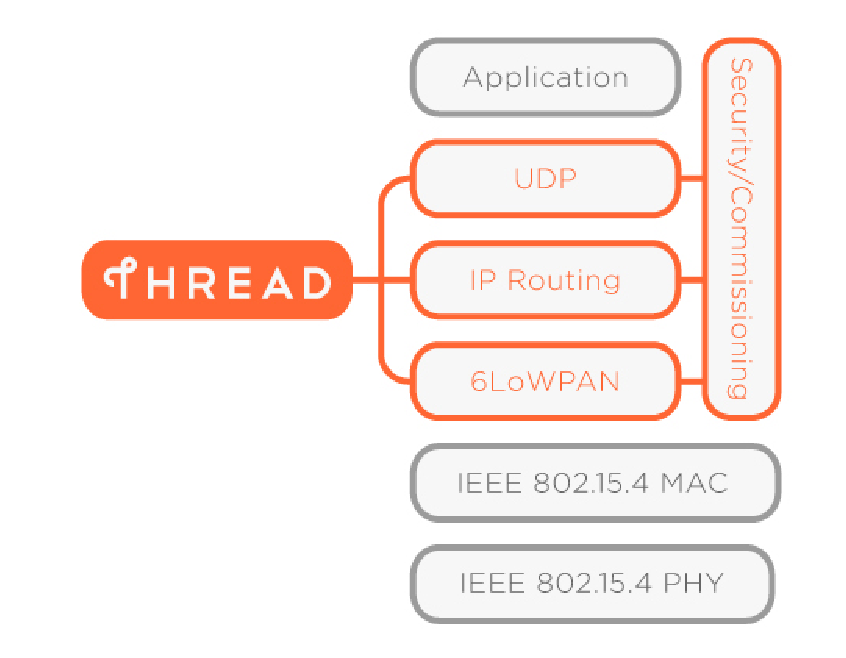
\includegraphics[width=9cm]{figuras/threadstack.eps}}
\caption{Pila del protocolo Thread  \cite{especificacionthread}}
\label{pilathread}
\end{figure}
\clearpage

\subsection{Características} % Caracteristicas
El protocolo Thread tiene una serie de características que lo diferencian del resto de soluciones IoT y lo convierten en uno de los protocolos para entornos domésticos más utilizados en domótica. Estas características son las siguientes:
\begin{itemize}
\item {\bf Instalación, arranque y funcionamiento de red simple}: la instalación de una red Thread es muy simple y se puede llevar a cabo utilizando un teléfono inteligente, una tableta o computadora. Los protocolos para formar y unirse a redes, permiten a los sistemas la autoconfiguración y solución de problemas de enrutamiento a medida que ocurren.
\item {\bf Redes domésticas y redes comerciales}: las redes domésticas pueden variar mucho en tamaño, de varios a cientos de dispositivos. Mientras que en las instalaciones comerciales, una sola red Thread no es suficiente para cubrir todos los requisitos de aplicación, sistema y red.
\item {\bf Protocolo seguro}: se implementa seguridad en la capa de red y se puede aplicar opcionalmente en la capa de aplicación. Thread ha sido diseñado para ofrecer la máxima seguridad en relación a la confidencialidad de las comunicaciones, garantizando que solo los dispositivos autorizados se unen a la red utilizando codigos de instalación de producto, encriptando todas las comunicaciones efectuadas. Para cerrar los agujeros de seguridad existentes en otros protocolos inalámbricos, se utiliza el estándar de encriptación AES y métodos de autenticación utilizados en smartphones.
\item {\bf Punto de fallo distibuido}: se utiliza un diseño de red de malla, conectando de forma segura diferentes dispositivos e impidiendo que haya un único punto de fallo. Si bien hay varios dispositivos en el sistema que realizan funciones especiales, Thread está diseñado para que se puedan reemplazar sin afectar el funcionamiento continuo de la red, siendo la reconfiguración invisible para el usuario. Sin embargo, bajo ciertas topologías habrá ciertos dispositivos individuales que no tengan capacidades de respaldo.
\item {\bf Alcance}: los dispositivos de la red proporcionan un rango de señal suficiente para cubrir un hogar normal.
\item {\bf Baja potencia}: tener como base el estándar IEEE 802.15.4 PHY/MAC asegura un consumo de energía extremadamente bajo. Además, los dispositivos de una red Thread se comunican de manera eficiente permitiendo que la vida útil de las baterías esperada en condiciones normales sea de varios años.
\end{itemize}
\clearpage




\subsection{Tipos de dispositivos} % Tipos de dispositivos
Una red Thread puede estar formada por los siguientes dispositivos:
\begin{itemize}
\item {\bf Router fronterizo}: es una puerta de enlace que proporciona conectividad para que la red Thread acceda a otras redes adyacentes como Wi-Fi, Ethernet, etc. Además, los routers fronterizos proporcionan servicios para dispositivos dentro de la red 802.15.4, incluidos los servicios de enrutamiento para operaciones fuera de la red. Una red Thread generalmente contiene uno o más routers fronterizos.
\item {\bf Dispositivo final elegible para router (REED)}: los REEDs son dispositivos que no actúan como routers de la red, no transmiten mensajes ni proporcionan servicios de unión o seguridad para otros dispositivos de la red, aunque tienen la capacidad de convertirse en routers si la red lo requiere. Los REEDs y los algoritmos de enrutamiento son administrados y promovidos por la red Thread sin intervención del usuario.
\item {\bf Líder}: es un dispositivo que administra un registro de los ids de routers asignados y acepta las peticiones de REEDs para convertirse en routers. Además, también asigna y administra las direcciones de los routers utilizando el protocolo de aplicación restringida (CoAP). Toda la información contenida en el líder está presente en los routers Thread. Por lo tanto, si el líder falla o pierde la conectividad, se elige automaticamente otro líder para la red.
\item {\bf Router Thread}: proporcionan los servicios de enrutamiento, unión y seguridad a los dispositivos de la red Thread. Estos dispositivos mantienen tablas de enrutamiento primarias y secundarias que se actualizan cuando un nodo deja de funcionar. Los routers Thread pueden actuar como líderes de la red y degradar su funcionalidad para convertirse en REEDs.
\item {\bf Dispositivo final}: los dispositivos finales que no son elegibles para routers (REEDs) pueden ser dispositivos finales completos (FED) o dispositivos finales mínimos (MED). La diferencia entre estos dispositios es que los MED no necesitan sincronizarse explícitamente con sus padres para comunicarse.
\item {\bf Dispositivo final dormido}: son dispositivos finales que se comunican solo a través de su padre (router Thread) y no pueden transmitir mensajes a otros dispositivos.
\end{itemize}
\clearpage



\subsection{Topologías de la red} % Topologías de la red
El tipo de topología de las redes Thread depende del número de routers que formen parte de la misma. Si solo hay un router, lo cual no es común, se forma una red en estrella. Sin embargo, si hay más de un router, se forma automáticamente una red en malla. De esta forma, el tipo de topología más utilizada en las redes Thread es la malla, lo que implica que en este tipo de redes IoT no hay un único punto de fallo.
\\\\
Las redes de malla integradas hacen que los sistemas sean más confiables al permitir que los nodos transmitan mensajes a otros nodos. Es decir, si un nodo no puede enviar un mensaje directamente, la red de malla transmite el mensaje a través de uno o más nodos intermedios. Para que la red en malla se mantenga y conecte constantemente, todos los nodos del router mantienen rutas y conectividad entre sí.
\\\\En este tipo de redes, se debe tener en cuenta que hay un límite de 64 direcciones de routers, permitiendo que las direcciones de los dispositivos eliminados sean reutilizadas, aunque no se pueden utilizar todas a la vez.
\\\\Existen dos tipos de redes Thread según la arquitectura utilizada para su formación:
\\\\$\blacksquare$ {\underline{\textbf{Arquitectura residencial}}} % Arquitectura Residencial
\\\\En una arquitectura residencial, el usuario o usuarios se comunican con la red residencial Thread desde su propio dispositivo inteligente (smartphone, tableta o computadora) a través de Wi-Fi en su red inalámbrica de área personal (WPAN) o mediante una aplicación basada en la nube. La siguiente figura muestra los tipos de dispositivos que forman este tipo de arquitectura.
\begin{figure}[H]
\centerline{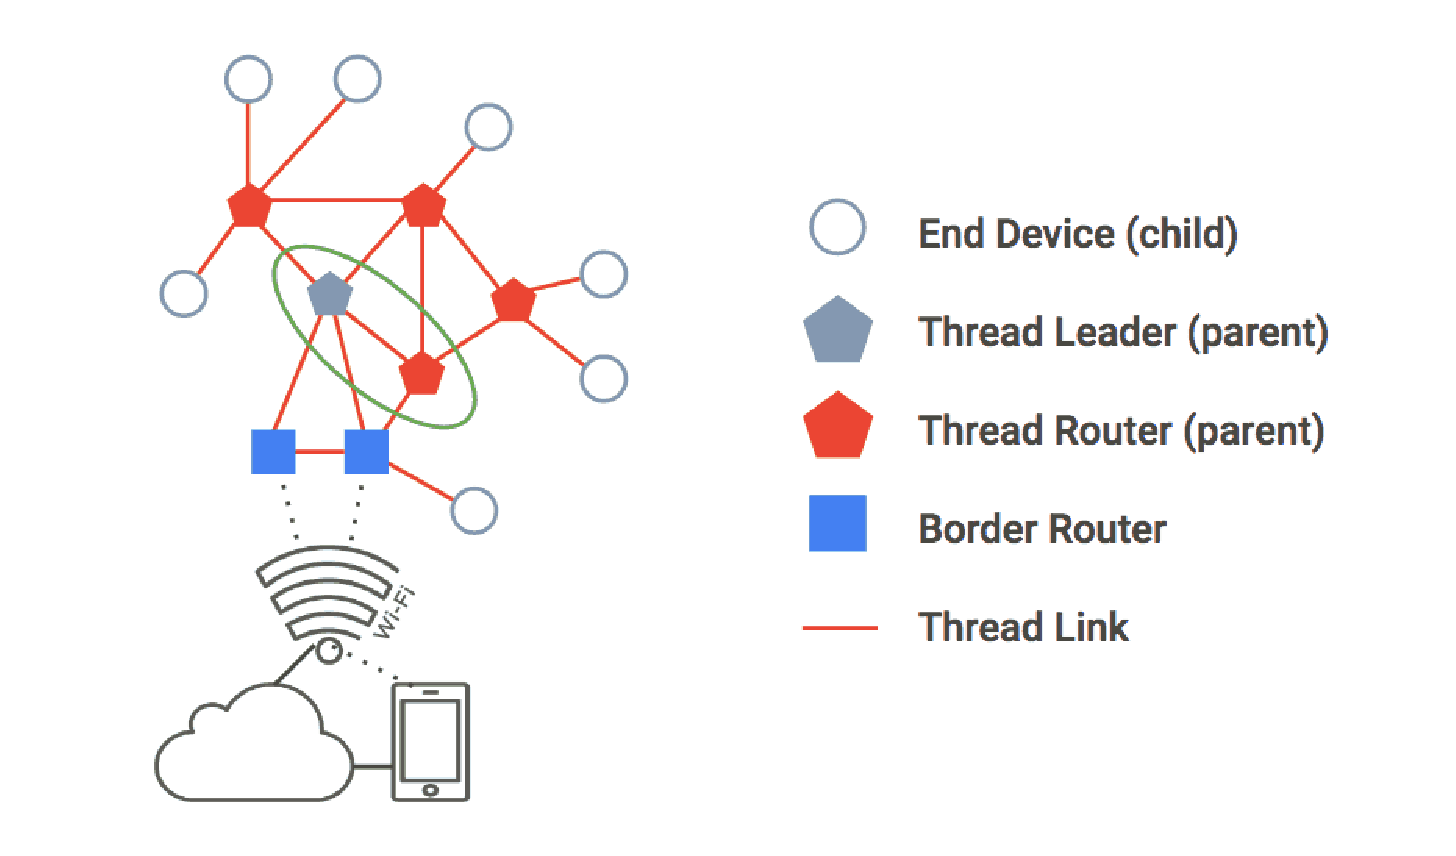
\includegraphics[width=9cm]{figuras/threadresidential.eps}}
\caption{Topología en malla (arquitectura residencial) \cite{threadtopologies}}
\label{topologiasthread}
\end{figure}
\clearpage




$\blacksquare$ {\underline{\textbf{Arquitectura comercial}}} % Arquitectura Comercial
\\\\En una arquitectura comercial, el usuario o usuarios se comunican con la red comercial Thread mediante un dispositivo inteligente (smartphone, tableta o computadora) a través de Wi-Fi o de la red empresarial. En este tipo de arquitectura, se utilizan los mismos dispositivos que en una red residencial aunque se agregan nuevos conceptos:
\begin{itemize}
\item {\bf Modelo de dominios Thread}: admite la integración de múltiples redes \\ Thread, así como una interfaz para redes IPv6 que no sean Thread. La principal ventaja de configurar una red con un dominio Thread común es que la unión de los dispositivos a cualquier red disponible es flexible, es decir, no hay planificaciones ni reconfiguraciones manuales cuando el tamaño de la red se amplía.
\item {\bf Router fronterizo troncal (BBR)}: son una clase de routers fronterizos existentes en las redes de área comercial que facilitan la sincronización del dominio Thread de múltiples segmentos de red y permiten la propagación de multidifusión de gran alcance dentro y fuera de cada malla. Una red Thread que es parte de un dominio más grande debe tener al menos un BBR ''primario'' y puede tener múltiples BBR ''secundarios'' para tener redundancia a prueba de fallos.
\item {\bf Enlace troncal}: es un enlace IPv6 (no Thread) al que se conecta un BBR mediante una interfaz externa que se utiliza para implementar el protocolo de enlace troncal Thread (TBLP), que permite la sincronización con otros BBR. Los dispositivos en una implementación comercial se configuran utilizando dominios Thread y direcciones únicas de dominio (DUA). El DUA de un dispositivo nunca cambia durante su vida útil al ser parte de un dominio Thread, lo que asegura que los respectivos BBR faciliten el enrutamiento y la migración a través de diferentes redes Thread.
\end{itemize}
\begin{figure}[H]
\centerline{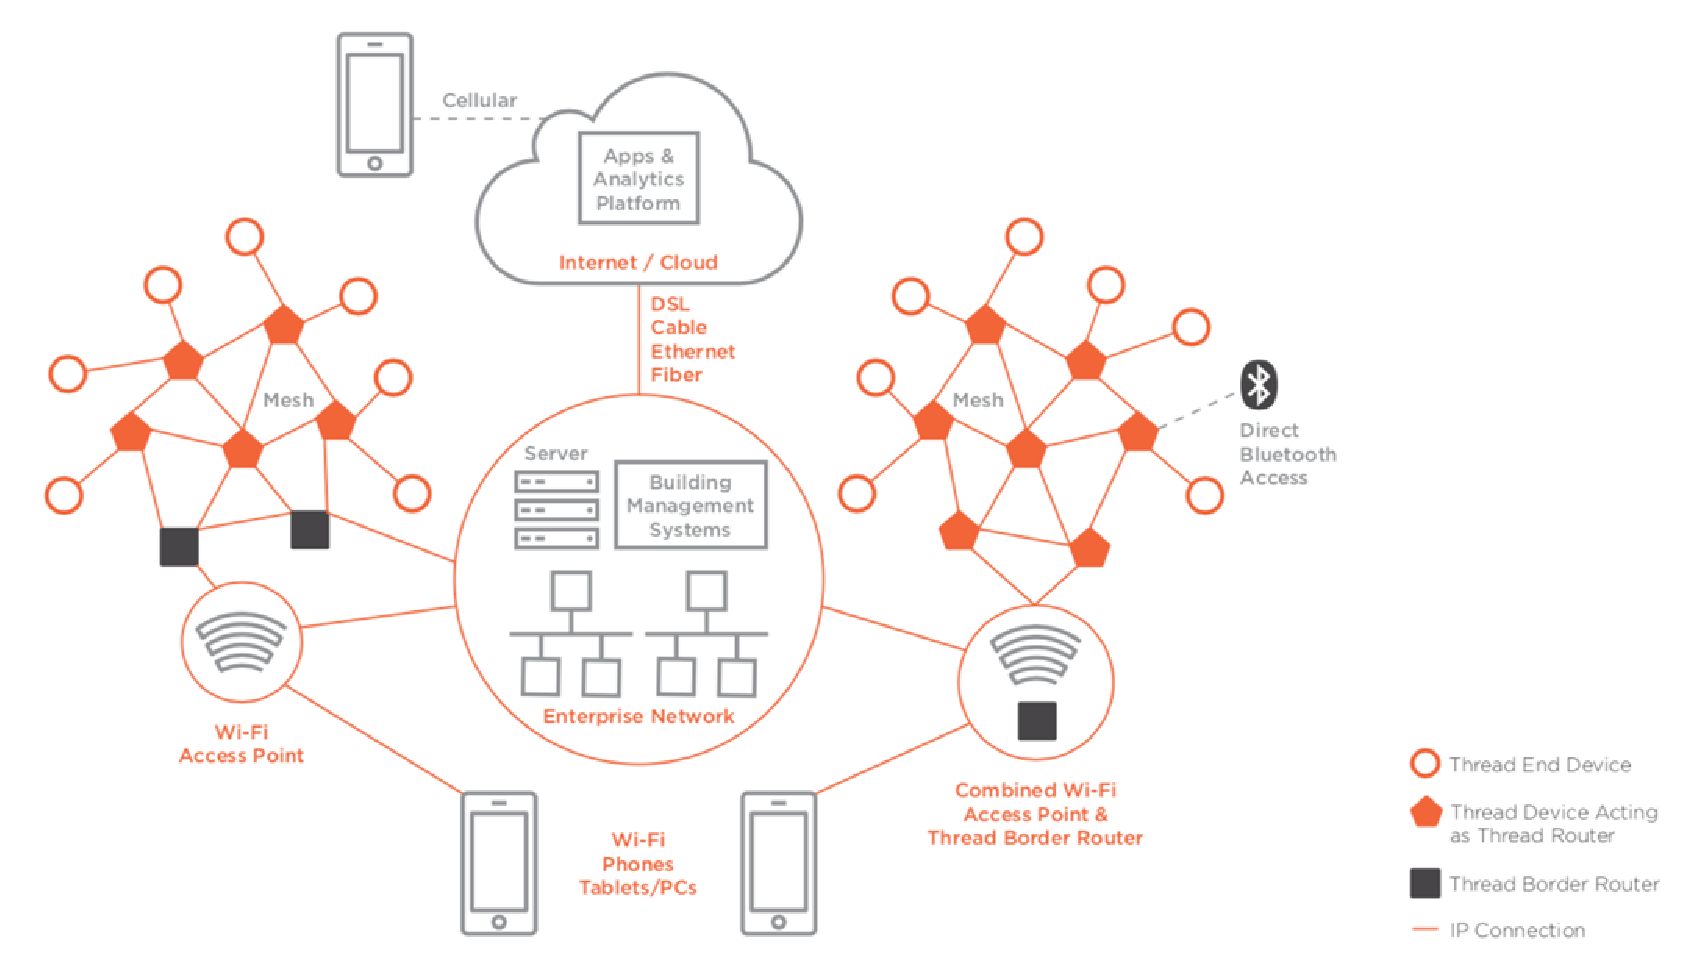
\includegraphics[width=13cm]{figuras/threadcomercial.eps}}
\caption{Topología en malla (arquitectura comercial) \cite{threadtopologies}}
\label{threadcomercial}
\end{figure}
\clearpage



\subsection{Arquitectura} % Arquitectura
Como se indicó anteriormente, Thread se basa en las capas física (PHY) y de control de acceso al medio (MAC) del estándar IEEE 802.15.4, construyendo a partir de ellas una especificación de capa de red y transporte que completan la pila del protocolo y añaden una serie de funcionalidades.
\subsubsection{Capa de red} % Capa de red
La capa de red que implementa Thread se fundamenta en los siguientes puntos:
\\\\$\blacksquare$ {\underline{\textbf{Direccionamiento IP}}} % Direccionamiento IP
\\\\Thread define la capa de red mediante una arquitectura de direccionamiento IPv6, direccionamiento de multidifusión y reenvío de paquetes. Esta arquitectura permite la configuración de una serie de direcciones que posibilitan el correcto funcionamiento de la red:
\begin{itemize}
\item Unique Local Address (ULA)
\item Domain Local Address (DUA)
\item Global Unicast Address (GUA)
\item Link-local all nodes multicast address
\item Link-local all routers multicast address
\item Solicited-node multicast address
\end{itemize}
\vspace{0.25cm}
A cada dispositivo que se une a la red Thread se le asigna una dirección corta de 16 bits. La dirección de los routers se asigna utilizando los bits de nivel superior, mientras que a los nodos hijo se les asigna una dirección utilizando los bits de nivel superior de sus padres y los bits más bajos apropiados para su dirección. Esto permite que cualquier dispositivo de la red comprenda la ubicación de enrutamiento de los nodos hijo simplemente al conocer los bits de nivel superior de su dirección.
\\\\
Los bits de nivel superior de una dirección IPv6 especifican la red y el resto especifican direcciones particulares en esa red. Por lo tanto, todas las direcciones de una red tienen los mismos primeros N bits. Esos primeros N bits se denominan prefijo o prefijo ULA (elegido por el dispositivo que inicia la red) indicando '/64' una dirección con un prefijo de 64 bits. El dispositivo que inicia la red Thread utiliza su dirección MAC para derivar su identificador de interfaz (IID) y generar una dirección IPv6 local de enlace con el conocido prefijo local fe80 :: 0/64.
\clearpage



$\blacksquare$ {\underline{\textbf{6LoWPAN}}} % 6LoWPAN
\\\\6LoWPAN, acrónimo en inglés de IPv6 sobre redes inalámbricas personales de baja potencia, es un estándar que posibilita el uso de IPv6 sobre redes basadas en IEEE 802.15.4. El objetivo principal de 6LoWPAN es transmitir y recibir paquetes IPv6 a través de enlaces 802.15.4. Aunque al hacerlo, tiene que adaptarse al tamaño máximo de trama enviada por el aire.
\\\\En los enlaces Ethernet, un paquete del tamaño de la unidad de transmisión máxima de IPv6 (MTU) (1280 bytes) se puede enviar fácilmente como una trama a través del enlace. Sin embargo, en el caso de 802.15.4, 6LoWPAN actúa como una capa de adaptación entre la capa de red IPv6 y la capa de enlace, resolviendo el problema de transmitir una MTU IPv6 al fragmentar el paquete en el remitente y reensamblarlo en el receptor. 6LoWPAN también proporciona un mecanismo de compresión que reduce los tamaños de encabezado IPv6 enviados y, por lo tanto, reduce la sobrecarga de transmisión.
\\\\
Otra característica importante de 6LoWPAN es que utiliza de la capacidad de reenvío de paquetes de la capa de enlace, sin tener que enviarlos a la capa de red. Thread hace uso de la capacidad de la capa MAC para proporcionar direccionamiento basado en direcciones cortas (16 bits) con el fin de reducir aún más los bits de información necesarios para proporcionar un reenvío de paquetes eficiente. Esto ahorra ciclos de procesamiento y mejora el consumo de energía sin dejar de utilizar un protocolo de enrutamiento basado en IP. 6LoWPAN posee esta capacidad ya que se ubica entre las capas 2 y 3 proporcionando los mecanismos e interfaces necesarias para su interconexión.
\\\\Thread hace un uso completo de este mecanismo para transmitir paquetes de manera eficiente a través de la red 802.15.4.

\subsubsection{Capa de transporte} %Capa de transporte
La pila de Thread soporta los protocolos UDP (User Datagram Protocol) y TCP (Transmission Control Protocol) para la transmisión de datos, aunque la implementación de este último es opcional:
\begin{itemize}
\item{\bf UDP}: se define para habilitar un modo de comunicación simple y sin conexión con conmutación de paquetes en un entorno de redes informáticas. UDP no garantiza la entrega ni la protección contra datos duplicados y asume que el protocolo de internet (IP) se utiliza como protocolo subyacente.
\item{\bf TCP}: se define para aplicaciones que requieren de una entrega fiable y ordenada de flujos de datos. El uso de este protocolo no es práctico en redes poco confiables o cuando la mayoría de los dispositivos están dormidos, es decir, cuando haya pocas transmisiones de datos entre los dispositivos.
\end{itemize}
\clearpage

\subsubsection{Fundamentos de las redes Thread} % Fundamentos de las redes Thread
$\blacksquare$ {\underline{\textbf{Formación de la red}}} % Formación de la red
\\\\Los dispositivos con la capacidad de formar una red son los router Thread y los router fronterizos. El proceso de formación comienza realizando una exploración de energía para identificar el canal menos ruidoso y luego se realiza una exploración activa, para identificar la lista de identificadores PAN que ya están en uso en ese canal. Posteriormente, el dispositivo debe elegir una lista de parámetros para la creación de la red: identificador PAN, nombre de la red, prefijo local de malla y credenciales de la red. El router también elige su propio ID y si la red está formada por un router fronterizo, la información de conexión externa se agrega a los datos de la red Thread.
\vspace{0.3cm}
\\\\$\blacksquare$ {\underline{\textbf{Unión de dispositivos}}} % Unión de dispositivos
\\\\Thread permite la unión de dispositivos a una red mediante dos métodos:
\begin{itemize}
\item Compartir la información de la red directamente con el dispositivo utilizando un método fuera de banda.
\item Establecer una sesión entre el dispositivo y una aplicación de administración de la red Thread, mediante un teléfono inteligente, tableta o interfaz web.
\end{itemize}
\vspace{0.25cm}
Los dispositivos que desean unirse a una red Thread realizan una petición de unión como dispositivos finales (MED, FED), dispositivos finales dormidos o como REEDs. Posteriormente, se inicia el proceso de enlace garantizando la privacidad de las comunicaciones mediante el protocolo DTLS y utilizando la clave preinstalada del dispositivo para autenticar de forma segura la unión.
\\\\Al final del enlace mediante DTLS, el líder comparte la clave KEK (explicada en el apartado \ref{seguridadredesthread}) con el dispositivo a unir, para posteriormente cifrar y enviar las credenciales de red (clave maestra, prefijo local de malla, contador de secuencia de la clave de red, identificador de la red, ..). Finalmente, cuando el dispositivo ya posee toda la información necesaria para comunicarse, se le asigna una dirección corta de 16 bits, generada a partir de la dirección del dispositivo padre. Esa dirección de red se utiliza para identificar al dispositivo y encaminar los datos hacia el mismo. Para que la asignación de direcciones no falle, el líder de la red cuenta con un mecanismo de distribución de direcciones que evita el asignar direcciones duplicadas a los nuevos dispositivos que se unen.
\\\\
A diferencia de los dispositivos finales, los REEDs luego de que se hayan unido y aprendido la configuración de la red, pueden solicitar convertirse en un router Thread, lo que causa que se les asigne otra dirección de red (dirección de router).
\clearpage




\subsection{Seguridad en redes Thread} % Seguridad en redes Thread
\label{seguridadredesthread}
Thread utiliza criptografía de clave simétrica para encriptar los mensajes de la red. El mecanismo de seguridad empleado en las redes Thread de malla consiste en los siguientes elementos de seguridad:
\begin{itemize}
\item {\bf Clave maestra}: es una clave secreta que se genera cuando se forma la red Thread. Esta clave se proporciona a todos los dispositivos en el proceso de unión a la red.
\item {\bf Clave de red}: es un código específico de la red que se genera cuando se forma y se utiliza para autenticar a un dispositivo candidato que quiere controlar la red Thread, es decir, el usuario de la red.
\item {\bf Clave del dispositivo}: es un código único preinstalado en cada dispositivo de la red Thread. Se utiliza durante la puesta en marcha del dispositivo para autenticar de forma segura la unión.
\item {\bf Clave de cifrado de la contraseña (KEK)}: es una clave derivada de la contraseña del dispositivo y se utiliza para distribuir de forma segura las credenciales de red a los dispositivo que se unen.
\item {\bf Clave MAC}: es una clave simétrica utilizada para cifrar mensajes en la capa MAC de la red Thread. Se deriva de la clave maestra utilizando un algoritmo de hashing y un contador de secuencia.
\item {\bf Clave MLE}: es una clave simétrica utilizada para proteger los mensajes del protocolo de establecimiento de enlace de malla. Se deriva de la clave maestra utilizando un algoritmo de hashing y un contador de secuencia. 
\item {\bf Credenciales de la red}: se refiere a la recopilación de datos específicos para unirse a la red como el prefijo IPv6, la clave maestra, el nombre de la red, etc.
\end{itemize}

\vspace{0.8cm}
La red Thread no tiene una seguridad centralizada. Sin embargo, es obligatorio actualizar periódicamente las claves MAC y MLE, utilizadas para cifrar mensajes entre nodos durante el funcionamiento de la red. Por lo tanto, cada nodo de la red realiza un procedimiento de actualización de claves que consta de dos pasos:
\begin{itemize}
\item Todos los nodos de la red generan una nueva clave.
\item Los nodos se sincronizan con sus vecinos más cercanos y todos los nodos modifican la clave.
\end{itemize}
Cada nodo consta de 3 claves MAC y 3 claves MLE (la clave anterior, la actual y la siguiente). Esta presencia de varias claves permite una migración sin problemas a la nueva clave. Sin embargo, no hay ningún método para cambiar la clave maestra durante el funcionamiento de la red.
